\documentclass[10pt]{report}
\usepackage[utf8]{inputenc}
\usepackage[italian]{babel}
\usepackage{multicol}
\usepackage[bookmarks]{hyperref}
\usepackage[a4paper, total={18cm, 25cm}]{geometry}
\usepackage{graphicx}
\usepackage{xcolor}
\usepackage{textcomp}
\graphicspath{ {./img/} }
\usepackage{listings}
\usepackage{makecell}
\usepackage{qtree}
\usepackage{pgfplots}
\usepackage{tikz}
\usepgflibrary{shapes}
\usepgfplotslibrary{fillbetween}
\definecolor{backcolour}{RGB}{255,255,255}
\definecolor{codegreen}{RGB}{27,168,11}
\definecolor{codeblue}{RGB}{35,35,205}
\definecolor{codegray}{RGB}{128,128,128}
\definecolor{codepurple}{RGB}{205,35,56}
\lstdefinestyle{myPython}{
	backgroundcolor=\color{backcolour},   
	commentstyle=\color{codegreen},
	keywordstyle=\color{codeblue},
	numberstyle=\tiny\color{codegray},
	stringstyle=\color{codepurple},
	basicstyle=\small\ttfamily,
	breakatwhitespace=false,         
	breaklines=true,                 
	captionpos=b,                    
	keepspaces=true,                 
	numbers=left,                    
	numbersep=2pt,                  
	showspaces=false,                
	showstringspaces=false,
	showtabs=false,                  
	tabsize=2,
	language=python
}
\newcommand*\triangled[1]{\tikz[baseline=(char.base)]{
            \node[regular polygon, regular polygon sides=3,draw,inner sep=1pt] (char) {#1};}}
            
\usepackage{fancyhdr}
\pagestyle{fancy}
\renewcommand{\headrulewidth}{0pt}
\fancyhead{}
\fancyfoot[L]{Telegram: \texttt{@fexed}}
\fancyfoot[R]{Github: \texttt{fexed}}
\begin{document}
\title{Parallel and Distributed Systems}
\author{Federico Matteoni}
\date{A.A. 2021/22}
\renewcommand*\contentsname{Index}

\maketitle
\tableofcontents
\pagebreak
\section{Introduction}
Prof.: Marco Danelutto
\paragraph{Program} Techniques for both parallel (single system, many core) and distributed (clusters of systems) systems.\\
Principles of parallel programming, structured parallel programming, parallel programming lab with standard and advanced (general purpose) \textbf{parallel programming frameworks}.
\paragraph{Technical Introduction} Each machine has more cores, perhaps multithreaded cores, but also GPUs (maybe with AVX support, which support operations floating point operations, \textbf{flops}, in a single instruction).\\
Between 1950 and 2000 the VLSI technology arised, integrated circuits which nowadays are in the order of 7nm (moving towards 2nm): printed circuits!\\
In origin, everything happened in a single clock cycle: fetch, decode, execute, write results in registers, with perhaps some memory accesses. The we had more complex control where in a single clock cycle we do just one of the phases (fetch \textit{or} decode \textit{or}\ldots), like a \textbf{pipeline}. More components are used the higher the frequency but the more power we need to dissipate, and we're coming to a point were the power we need to dissipate is too much and risks to melt the circuit, so we're reaching a \textbf{physical limit} in chip miniaturization. But temperature and computing power do not go in tandem: computing power is proportional to the chip dimensions, while temperature is proportional to the area. So it's better to put more processors (\textbf{cores}) and let them work together rather than make a bigger single processor.\\
An approach is to have few powerful cores and more less powerful cores (for example, in the Xeon Phi processors). Now, the processors follow this architecture, with the performance of a single core decreasing a bit with every generation but it's leveled by adding more cores.\\\\
Up to the 2000, during the single core era, code written years before will run faster on newer machines. Now, code could run slower due to not exploiting more cores and the decreasing in performance of the single core.\\With accelerators the situation is even more different: for example GPUs, accelerator for graphics libraries, with their own memory and specialized in certain kinds of operations. This can require the transfer of data between the accelerator's memory and the main memory, so the architecture of the accelerator is impactful on the overall performance.
\section{General Paradigms of Parallel Programming}
\paragraph{Parallelism} Execution of different parts of a program on different computing devices at the same time. We can imagine different flows of control (sequences of instruction) that all together are a program and are executed on different computing devices. Note that more flows on a singe computing device is \textbf{concurrency}, not parallelism.
\subparagraph{Concurrency} Similar concept: things that \textit{may} happen in parallel respecting the ordering between elements.
\paragraph{Computing Devices}\begin{list}{}{}
	\item \textbf{Threads}, implying shared memory
	\item \textbf{Processes}, implying separated memories
	\item \textbf{GPU Cores}
	\item \textbf{Hardware Layouts} on a FPGA (Field Programmable Gate Array) 
\end{list}
\paragraph{Sequential Task} A "program" with its own input data that can be executed by a single computing entity
\paragraph{Overhead} Actions required to organize the computation but that are note included in the program. For example: time spent in organizing the result. Basically, time spent orchestrating the parallel computation and not present in the sequential computation.
\paragraph{Speedup} Fundamental things that we're looking for, it's the ratio between the sequential time and the parallel time.$$\hbox{SpeedUp} = \frac{\hbox{Sequential time}}{\hbox{Parallel time}}$$
Assuming the best sequential time.\\
We have a slightly different measure, too
$$\hbox{Scalability}=\frac{\hbox{Parallel time with 1 computing device}}{\hbox{Parallel time}}$$
\paragraph{Stream of tasks} In some cases it's not important considering just one computation but may be useful considering more computations and we want to optimize a set of tasks.
\paragraph{Example: Book Translation} With $m=600$ pages, for example. Let's assume I can translate a page in $t_p = 0.5$h.\\
The sequential task is: take the book and spend time until I can deliver the translated book. The time is circa $m\cdot t_p = 300$h.\\
In parallel, ideally every page can be translated independently so I can split the book in two pieces of $\frac{m}{2}$ pages each (overhead), giving each half to a person. Both can translate at the same time, so ideally the time required is $\frac{m}{2}\cdot t_p$ for each, producing the translated halves. At this point I get the halves and produce the translated version (overhead). Ideally the time require is more or less $\frac{m}{2}\cdot t_p$, with "more or less" given by the time spent in splitting the book and reuniting the two halves. So the exact time is $T = T_{split} + \frac{m}{2} \cdot t_p + T_{merge}$.\\
What if the two person have different $t_p$s? For example $t_1 > t_2$. When a translator finishes, it spends some time synchronizing its work with me. With $nw$ "workers" (translators, in this instance) $T = nw\cdot T_{split} + nw\cdot T_{merge} + \frac{m}{nw}T_{work}$ with $nw\cdot T_{split}$ time spent delivering work to each worker and $nw\cdot T_{merge}$ time in merging each result.\\\\
Init is the time where every worker has work to do, and finish is the time where the last worker finished working. So the exact formula is with a single $T_{merge}$.\\
So $\frac{m}{nw}T_{work}$ is the time that needs to happen, found in the sequential computation too, whereas the other two factors are \textbf{overhead}.
$$\hbox{SpeedUp} = \frac{\hbox{Best sequential time}}{\hbox{Parallel time}}$$ but the parallel time depends on the $nw$ so $$\hbox{SpeedUp}(nw) = \frac{\hbox{Best sequential time}}{\hbox{Parallel time}(nw)} \simeq \frac{\not m\cdot \not t_p}{\frac{\not m}{nw}\cdot \not t_p} = nw$$ This not taking into account the overhead. It's a realistic assumption because usually the time splitting the work is very small. But we have to take into account that, in case it's not negligible. $$\hbox{SpeedUp}(nw) = \frac{m\cdot t_p}{\frac{m}{nw}\cdot t_p + \underline{nw\cdot T_{split} + T_{merge}}}$$
%TODO graph sp(nw) over (nw)
\paragraph{Example: Conference Bag} $T_{bag} = t_{bag} + t_{pen} + t_{paper} + t_{proc}$ and with $m$ bags we have $T = m\cdot T_{bag}$\\
We could build a pipeline, a building chain, with 4 people and each person does one task: \begin{list}{}{}
	\item One takes the bag and gives to the next
	\item One puts the pen into the bag and passes it
	\item One puts the paper into the bag and passes it
	\item One puts the proceedings into the bag
\end{list}
So $w_b, w_{pen}, w_{paper}, w_{proc}$ workers. When the first worker has passed the bag, it could begin taking the next bag. Same for the others.
\begin{center}
	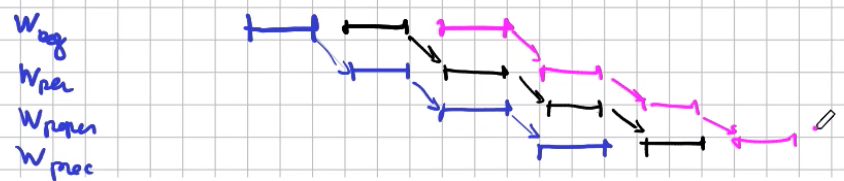
\includegraphics[scale=0.5]{1.png}
\end{center}
So in sequential we have $m\cdot(t_{bag} + t_{pen} + t_{paper} + t_{proc})$, and in parallel per 1 bag we have $t_{bag} + t_{comm} + t_{pen} + t_{comm} + t_{paper} + t_{comm} + t_{proc} + t_{comm}$ with $t_{comm}$ spent passing the bag from one to the other, so total of $m\cdot T_{seq} + m\cdot t_{comm}$. But that's not correct, because we work in parallel: ideally we have a parallelogram of $m\cdot(t_{proc} + t_{comm}$ base, and we require $t_{bag} + t_{pen} + t_{paper} + 3\cdot t_{comm}$ time to get up to speed and "fill the pipeline". But this required time is negligible, and in the end the overall time is given by the base of the parallelogram.
\paragraph{Pipeline} With $m$ tasks and $nw$ stages, with the completion of the stage $i$ required in stage $i+1$. So the output is $f_{nw}(f_{nw-1}(\ldots f_1(x_i)\ldots))$. With $t$ time required for each stage.
\begin{center}
	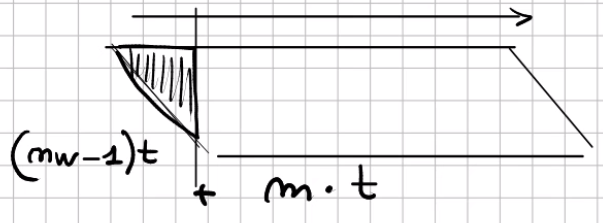
\includegraphics[scale=0.5]{2.png}
\end{center}
We spend $(nw-1)t$ to get the last stage working and $m\cdot t$ time spent by the last stage to complete all the tasks.
$$T_{par}(nw) = (nw-1)\cdot t + m\cdot t$$
$$\hbox{SpeedUp}(nw)=\frac{(nw\cdot t)\cdot m}{(nw-1)\cdot t + m\cdot t}$$
So the higher the $m$ is, the lower is the impact of the time required to get up to speed. So $m >> nw \Rightarrow T_{par}(nw) \simeq m\cdot t$
\paragraph{Throughput} Tasks completed per unit of time.
\section{Measures}
On one side we can have more speed with more resources (computing devices). On the other side we can use more complex applications, with more resources. For example more precise computations, so extra resources not for improving the time but to improve the quality of the computations.\\
Finally, we could aim at computing results with less energy thanks to parallelism. This is a recent perspective on parallelism.\\\\
We've seen the SpeedUp($n$) = $\frac{T_{seq}}{T_{par}(n)}$, where the plot has to lie below the bisection of the cartesian graph.
\subsection{Base Measurements}
\paragraph{Latency $L$} Measure of the wall-clock time between the start and end of the single task.
\paragraph{Service Time $T_s$} It's related to the possibility of executing more tasks. It's the measure of the time between the delivery of two consecutive results, for example between $f(x_i)$ and $f(x_{i+1})$\\
Even if $x_i$ and $x_{i+1}$ arrive at the same time, $f$ would still be computing $f(x_i)$ so it'll start computing $f(x_{i+1})$ when it has finished.
\paragraph{Completion Time $T_c$} The latency related to a number of tasks. $T_c = L\cdot m$ for $x_m,\ldots,x_1$ inputs to a sequential system.\\
With a parallel system, instead, we have $T_c\simeq m\cdot T_s$.
\paragraph{Example} A 3 stage pipeline, with each node being sequential and with latency $L_i$ for node $i$.\\
At $t_0$ the first stage $N_1$ gets the first tasks and computes it in $L_1$, then $N_2$ computes in $L_2$ and $N_3$ computes in $L_3$ so a total of $t_0 + L_1 + L_2 + L_3$.\\
When the pipeline is filled, $T_s$ is dominated by the longest $L_i$, so $T_s = \max\{L_1, L_2, L_3\}$ and $T_c = \sum L_i + (m-1)T_s$\\
If $m$ is large with respect to $n=$ number of stages, the "base of the parallelogram" would be very long, so $m >> n \Leftrightarrow T_c = m\cdot T_s$
\subsection{Derived Measurements}
\paragraph{SpeedUp} $$\hbox{SpeedUp}(n) = \frac{T_{seq}}{T_{par}(n)}$$ Could be latencies, service times\ldots depending on what we want to measure the speedup of.
\paragraph{Scalability} $$\hbox{Scalability}(n)=\frac{T_{par}(1)}{T_{par}(n)}$$
\paragraph{Efficiency} $$\hbox{Efficiency}(n) = \frac{\hbox{Ideal parallel time}(n)}{T_{par}(n)} = \frac{\frac{T_{seq}}{n}}{T_{par}(n)} = \frac{T_{seq}}{n\cdot T_{par}(n)} = \frac{\hbox{SpeedUp}(n)}{n}$$
Measures the tradeoff between what you gain with the speedup and the cost of the speedup.
\paragraph{Throughput} $$\hbox{Throughput} = \frac{1}{T_s}$$
\paragraph{Amdahl Law} Taken the total time of a computation, $T_{seq}$, it can be divided into something that can and something that cannot be computed in parallel (for example, dividing the book is a sequential activity). So we can say that\\$T_{seq} =$ serial fraction + parallel fraction and the \textbf{serial fraction cannot be parallelized}. $f\in[0,1]\:|\:f\cdot T_{seq}$ is the serial fraction.
$$T_{seq} = f\cdot T_{seq} + (1-f)\cdot T_{seq}$$
The parallel fraction can be splitted between the workers, but we would have to compute the serial fraction too. By splitting more and more and more, we have that $$\lim_{n\to\infty} T_{par}(n) = f\cdot T_{seq}$$ $$\hbox{SpeedUp}(n) = \frac{T_{seq}}{f\cdot T_{seq}} = \frac{1}{f}$$
So we have a very low upper bound on the achievable speedup. This is referred to as \textbf{strong scaling}: strong meaning using more resources to get the computation faster.
\paragraph{Gustaffson Law} $$\hbox{SpeedUp}(n) = N - S\cdot(N-1)$$ With $S$ being the serial fraction. This comes from the fact that we're considering a different perspective: Gustaffson assumes that the computation increases with the parallelism, something that's called \textbf{weak scaling}, getting the speedup from using more computational devices, using more data. %TODO rivedere 17/02 inizio parte 2
\paragraph{Cores} In modern computers, we have a main memory (slow), a disk (even slower) and the memory is connected to at least 3 levels of cache. At the bottom we have some cores (4, 8\ldots), each one has its own level 1 cache (usually split in data and instruction cache).\\
With an activity with a working set that fills the cache, in case of strong scaling splitting the computation across cores we process less data per core because the size of the problem is the same.\\
With weak scaling, we assume that the data increases so by using more cores we process the same data on all cores but the data grows so we could have extra overhead because of the working set size.\\
We will have patterns of parallel computation that differentiate in how we process the data.
\paragraph{Application as Graphs} The applications can be seen as graphs of sequential nodes with dependencies.
%TODO
The maximum speedup is the work over the span, because in every case I need to go from the first to the goal node. I take the longest one because at least the longest path must be computed, and all the rest can be done in parallel and I assume to have enough resources to compute the rest in the time of the span.\\
We can use this model %TODO
\section{Technicalities}
\paragraph{Examples}
A simple program that "translates" an ASCII file by transforming lower letters into capital letters. We split the text into $n_{workers}$ parts, we wait for all the threads to finish and then verify the performances.
\\The translator is:
\begin{lstlisting}[style=myPython]
#include <string>

char translate_char(char c) {
	if (islower(c))
		return(toupper(c));
	else
		return(tolower(c));
}
\end{lstlisting}
%TODO
\subsection{Threads}
We used to write instructions sequentially. At a given point now we \texttt{fork} another flow of computation: we get two flows that are executed together \textbf{in the same address space}, so the new thread inherits all the memory of the original thread.
\paragraph{Concurrence} \texttt{todo} %TODO
\section{Patterns}
Computations with particular shapes and semantics that can be understood and implemented depending on the situations, not linked to languages and technicalities. Patterns are a useful concepts, allow programmers to reuse experience of other programmers an not reinventing the wheel.\\
Parallel patterns:
\begin{list}{}{}
	\item Data parallel
	\item Stream parallel
\end{list}
The same patterns can be referred with different names.
\subsection{Data Parallel Patterns}
Parallelism comes from data: we split the data in pieces, compute a set of results that can be combined into a single final result. The book translation examples is a data parallel pattern. What matters is $L$.\\
The general pattern is:
\begin{list}{}{}
	\item Decomposition
	\item Partial results
	\item Recomposition
\end{list}\begin{multicols}{2}
\subparagraph{Map Pattern} Also called applytoall:\begin{list}{}{}
	\item $\forall$ item of the collection
	\item Function $f($item$)$
	\item $\forall$ $f($item$) \rightarrow$ isomorphic collection
\end{list}
\subparagraph{Reduce Pattern} Also called fold:\begin{list}{}{}
	\item $\forall$ item of the collection
	\item $\oplus(x,y)$
	\item $\oplus(\oplus(a,b),\oplus(c,d))$
\end{list}
\end{multicols}
\subparagraph{Stencil Pattern} \begin{list}{}{}
	\item In partially overlapping position, e.g. of a matrix or an image
	\item Function $f($item$)$
	\item $\forall$ $f($item$) \rightarrow$ isomorphic collection
\end{list}
Different kind of problems: overlapping positions will yield the new value, so we have to account for that.
\subparagraph{"Google" mapreduce}
\begin{list}{}{}
	\item $\forall$ items
	\item $f($item$) + \oplus($item$, $item$)$
	\item Item
\end{list}
What I apply to each item is an $f$ that maps to $\langle$key, value$\rangle$ and $\oplus$ applies the sum to each value.\\
For example in a document, $f($word$)=\langle w,1\rangle$ and $\oplus(\langle w_k,v_1\rangle,\langle w_k,v_2\rangle) = \langle w_k, \oplus(v_1,v_2)\rangle$\\
"The lesson given by the professor", $f$ will output $\langle$the, 1$\rangle,\langle$lesson, 1$\rangle$\ldots and $\oplus$ will for example output $\langle$the, 2$\rangle$.\\
We can apply the map function over all the data distributed in various databases, for example.\\
This is \texttt{map(f)} and \texttt{reduce($\oplus$)}, but we want something like \texttt{map(reduce($\oplus$))}. Combining elementary patterns to achieve more complex results. Like two nested \texttt{for}s.\\
So I want building blocks, something that guarantees correctness of implementation that can be used to build upon. For example \texttt{map(function<A(B)>, collection<B>)}\\
So build a bag of tools that we can combine to undertake common situations with good efficiency, speedup, scalability\ldots
\subsection{Stream Parallel Patterns}
Stream of data, flowing in time. In data parallel we process a data collection, while in stream parallel we don't have data appearing all at the same time. So stream as a collection with items appearing at different times. We want to take the single items and try to process in parallel, parallel execution of $f$ over different items of the stream.\\
What matters is $T_S$
\paragraph{Pipeline}
\begin{center}
	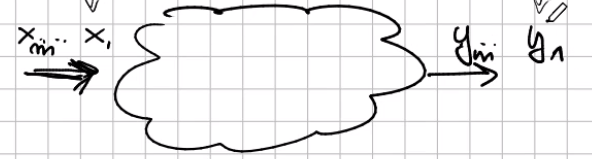
\includegraphics[scale=0.5]{3.png}
\end{center}
Inside the pipeline we have $f_1\rightarrow f_2\rightarrow\ldots\rightarrow f_k$ with each $f_i$ corresponding to a phase, with $f_i$ taking input from $f_{i-1}$.\\
So $x_i\mapsto f_1(x_i)\mapsto f_2(f_1(x_i))\mapsto \ldots$, and the parallelism is in the computation of different phases of different items (much like what we've seen with the CPU fetch-decode-execute pipeline).
\begin{center}
	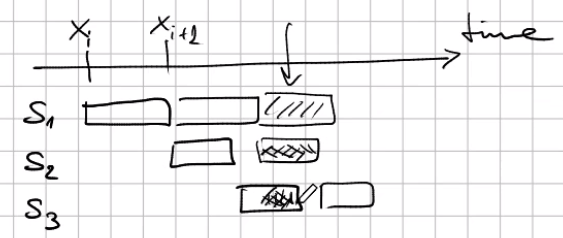
\includegraphics[scale=0.5]{4.png}
\end{center}
\paragraph{Farm}
We have a number $nw$ of instances of the same function $f$ each processing one single item.
\begin{center}
	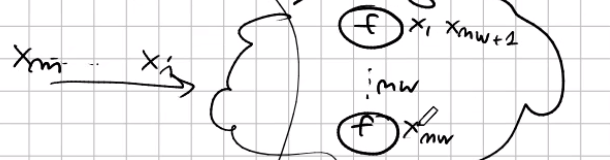
\includegraphics[scale=0.5]{5.png}
\end{center}
We have no interference between computations of $x_i,x_j$ with $i\neq j$, no need for synchronization.
\paragraph{} $T_C \simeq m\cdot T_S$ and $T_S$ in sequential is $\simeq L$ this means that I can try to decrease the latency by decreasing the stages in the pipeline or the workers in a farm.
\paragraph{Two Tier Model} Let's assume a grammar of patterns.\begin{list}{}{}
	\item Pat = Seq(f) $|$ DPP $|$ SPP
	\item DPP = Map(Pat) $|$ Reduce(Pat)
	\item SPP = Farm(Pat) $|$ Pipe(Pat, Pat)
\end{list}
This defines parallel computations and we aim at assuring that this can be done, a way of implementing this. So\begin{list}{}{}
	\item Map(Pipe(Seq(f), Seq(g)))
\end{list}
can be a data parallel computation where on the single item we compute a 2-stages pipeline of $f$ and $g$. But each element of the map is given to a single pipeline, or each pipeline receives a single item, so the stream parallelism is useless.
\begin{list}{}{}
	\item Farm(Map(Seq(f)))
\end{list}
Here we have a stream of items that will be processed by a Farm, each item splitted by Map and processed. This can deliver the result faster and access the next item.\\
So Data parallel with Stream parallel is not very good, Stream parallel with Data parallel is better: \textbf{two tier model}.\\
So we have an initial part of the pattern which is Stream Parallel, the second part is Data Parallel and eventually the last stages (the leafs of the tree) which are sequential.
\subsection{Parallel Design Patterns}
Also called \textbf{algorithm skeletons}: programming abstraction that model some pattern. The programmer has a framework, libraries, languages and that includes algorithm abstractions.
\end{document}